\chapter{破缺的对称性、戈德斯通玻色子与规范不变性}

我们想要理解一个类光子粒子如何能够获得质量。那是目的地，但它并不是一个合理的出发点。规范场的直接质量项似乎会破坏使理论自洽的规范不变性本身。在我们能够看到出路之前，我们需要以可操作的形式掌握两个概念：
\begin{enumerate}
  \item 自发对称破缺，特别是对于连续对称性；
  \item 规范不变性，其中对称操作可以从一个时空点到另一个时空点变化。
\end{enumerate}
这两个概念都不能用一句口号来代替。我们将从一块磁体出发构建第一个概念，将其翻译成标量场论，并发现无质量的戈德斯通模式。然后我们将取同一个\(U(1)\)对称性并使其局域化，这迫使我们引入矢量势和协变导数。只有在最后，这两条线索才会被并排放置。它们实际的结合---希格斯现象---是下一讲的主题。

\section{具有不对称基态的对称定律}

\subsection{两态磁体}

从一个小磁体的点阵开始。每个自旋可以指向上或下，相邻自旋通过指向相同方向来降低能量。在三维立方点阵上，一个自旋有六个最近邻，但精确的配位数并不重要。重要的是规则
\begin{equation}
  E_{\parallel}<E_{\rm antiparallel}.
\end{equation}
如果每个自旋都反转，微观规则保持不变：
\begin{equation}
  \uparrow\longleftrightarrow\downarrow.
\end{equation}
然而，最低能量的构型本身并不对称。它们是
\begin{equation}
  \{\uparrow\uparrow\uparrow\cdots\},
  \qquad
  \{\downarrow\downarrow\downarrow\cdots\}.
\end{equation}
方程允许两者，但一个冷的宏观样品必须选择其一。

这种选择极其敏感。将远处的一个自旋固定为指向上。它的邻居倾向于跟随它，邻居的邻居倾向于跟随它们，信息通过样品传播。与整个系统相比任意小的微扰可以选择整个基态的取向。这就是\emph{自发}对称破缺所指的不稳定性。

\begin{classroomqa}
\audiencequestion{中性粒子能在磁场中定向吗？
\lecturetimestamp{00:05:14}}
\lecturerresponse{能。电中性并不意味着没有磁矩。中子是中性的，但由于其内部带电组分而具有磁矩。因此磁场可以区分其自旋取向。}
\end{classroomqa}

\begin{classroomqa}
\audiencequestion{如果系统改变取向，变化是同时发生在所有地方吗？几个重新取向的波可以共存吗？
\lecturetimestamp{00:05:41--00:06:38}}
\lecturerresponse{变化会传播。一个区域推倒它的邻居，就像三维多米诺骨牌阵列一样，扰动以波的形式传播。不同区域可以独立地开始选择，因此在一种取向获胜之前，可能存在几个前沿和几个畴。当对称性变为连续时，我们将回到正是这些波。}
\end{classroomqa}

\subsection{显式破缺是不同的理论}

现在将样品置于指向上方的外磁场中。一个孤立自旋在指向上时已经具有较低能量。变换\(\uparrow\leftrightarrow\downarrow\)不再保持能量不变：偏好已被插入定律本身。这就是\emph{显式}对称破缺。

这种差异可以在不知道样品如何制备的情况下被检验。取一个非常大的样本，保持其左边界向上，保持其右边界向下。如果体磁场显式地偏好向上，右手约束只能穿透很短的距离。一个宏观的向下区域将付出与其体积成正比的能量，因此体相不能保持分裂为两个同样好的相。

没有外部偏置时，向上和向下具有相同的体能量。最低能量的约束态则包含一个向上畴、一个向下畴以及它们之间的有限过渡层。界面不必位于几何中心，但没有体积压力迫使一个相抹去另一个相。这个界面是一个\emph{畴壁}，是这种破缺离散对称性的特征缺陷。

\begin{figure}[htbp]
\centering
\begin{adjustbox}{max width=\linewidth}
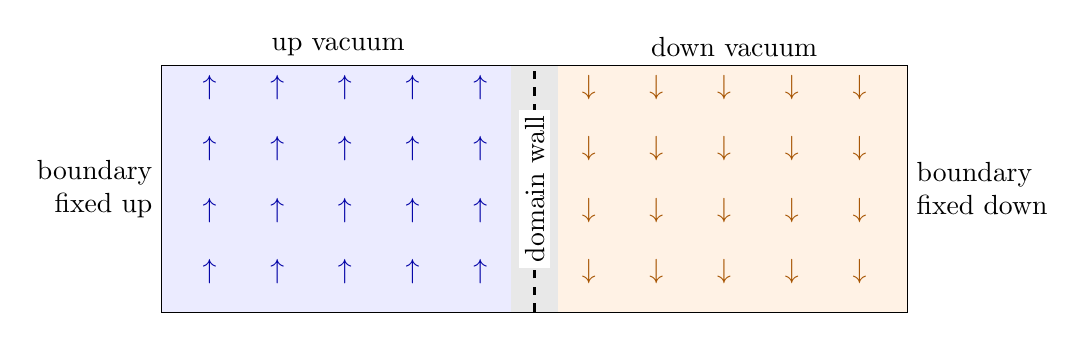
\begin{tikzpicture}[x=0.86cm,y=0.78cm]
  \draw[thick] (0,0) rectangle (11,4);
  \fill[blue!8] (0,0) rectangle (5.15,4);
  \fill[orange!10] (5.85,0) rectangle (11,4);
  \fill[gray!18] (5.15,0) rectangle (5.85,4);
  \foreach \x in {0.7,1.7,2.7,3.7,4.7}
    \foreach \y in {0.65,1.65,2.65,3.65}
      \node[blue!65!black] at (\x,\y) {$\uparrow$};
  \foreach \x in {6.3,7.3,8.3,9.3,10.3}
    \foreach \y in {0.65,1.65,2.65,3.65}
      \node[orange!65!black] at (\x,\y) {$\downarrow$};
  \draw[dashed,thick] (5.5,0) -- (5.5,4);
  \node[above] at (2.6,4) {up vacuum};
  \node[above] at (8.45,4) {down vacuum};
  \node[rotate=90,fill=white,inner sep=2pt] at (5.5,2) {domain wall};
  \node[left,align=right] at (0,2) {boundary\\fixed up};
  \node[right,align=left] at (11,2) {boundary\\fixed down};
\end{tikzpicture}
\end{adjustbox}
\caption{离散对称性自发破缺的边界检验。两种体取向具有相同的能量，因此壁可以分隔宏观畴。}
\end{figure}

\begin{classroomqa}
\audiencequestion{这个论证是否只要求最近邻之间的相互作用？\lecturetimestamp{00:18:18}}
\lecturerresponse{不。次近邻相互作用如果也倾向于排列一致，会改变细节，但不会改变结论。如果不同作用范围相互竞争，就会出现更有趣的行为---例如，最近邻倾向于排列一致，而次近邻倾向于反排列。这会产生阻挫和更复杂的有序相，但不会改变这里所作的基本区分。}
\end{classroomqa}

\begin{classroomqa}
\audiencequestion{\emph{自发}指的是畴壁内部的大导数吗？\lecturetimestamp{00:19:05}}
\lecturerresponse{不。它指的是这样一个事实：底层能量没有上--下的偏好，而所选定的基态却有。对任意小扰动的剧烈响应揭示了一种不稳定性。梯度仅仅告诉我们界面的代价有多大。}
\end{classroomqa}

\begin{classroomqa}
\audiencequestion{该材料已经处于两种状态之一，还是其状态最初未知？\lecturetimestamp{00:19:40}}
\lecturerresponse{这取决于它的历史。在高温下，热运动可以使自旋向上和向下混合，平均磁化强度几乎为零。随着材料冷却，不同区域选择不同取向，畴壁形成，畴逐渐粗化。偶然性和微小的环境扰动决定了最终哪个真空占据样品的大部分。}
\end{classroomqa}

\section{与标量场论相同的论证}

用实标量场\(\phi(\bm{x},t)\)代替自旋。在度规和归一化约定一经固定之后，写出
\begin{equation}
\begin{aligned}
  \mathcal L
  &=\frac12\,\partial_\mu\phi\,\partial^\mu\phi-V(\phi),
  \\
  \mathcal E
  &=\frac12\dot\phi^{\,2}+\frac12(\nabla\phi)^2+V(\phi).
\end{aligned}
  \label{eq:l07-real-scalar}
\end{equation}
\(\mathcal L\)中的相对论性简写包含正的时间导数项和负的空间梯度项；哈密顿量能量密度中这两项贡献都为正。

选择一个具有两个简并极小值的偶势，
\begin{equation}
  V(\phi)=\frac{\lambda}{4}\left(\phi^2-f^2\right)^2,
  \qquad \lambda>0.
  \label{eq:l07-double-well}
\end{equation}
拉格朗日量在\(\phi\mapsto-\phi\)下不变，而任一均匀真空
\begin{equation}
  \phi(\bm{x})=+f,
  \qquad\hbox{or}\qquad
  \phi(\bm{x})=-f
\end{equation}
选择一侧。相比之下，在\(\phi=0\)处具有唯一极小值的势具有对称真空，不发生自发破缺。

将样品一侧的\(\phi=+f\)和另一侧的\(\phi=-f\)固定。场不可能无代价地跳跃，因为
\begin{equation}
  E_{\rm wall}
  =\int dx\left[
      \frac12\left(\frac{d\phi}{dx}\right)^2+V(\phi)-V(f)
    \right].
  \label{eq:l07-wall-energy}
\end{equation}
突然跳跃会使\(d\phi/dx\)变得极大。因此，最小能量的畴壁将变化展布在有限宽度上，在梯度能量与穿越极小值之间的势能代价之间取得平衡。式~\eqref{eq:l07-double-well}中势的熟悉扭结解为
\begin{equation}
  \phi_{\rm wall}(x)
  =f\tanh\!\left[f\sqrt{\frac{\lambda}{2}}\,(x-x_0)\right],
  \label{eq:l07-kink}
\end{equation}
这是黑板上所述平滑过渡的一个显式实现。
\editorialnote{讲座根据势的形状和梯度项进行论证，但并未求解场方程。方程
\eqref{eq:l07-kink}作为该所述模型的标准解被纳入，使定性的畴壁具体化，而不改变论证。}

将双势阱稍微倾斜，一个极小值就变得较低。此时拉格朗日量本身不再对称。畴壁仍可暂时出现，但较高能量的真空或假真空会对其施加压力；畴壁移动，受偏好的相膨胀。这是外磁场导致显式破缺的场论版本。

到目前为止，对称性都是离散的。粒子物理学由连续群主导，例如\(U(1)\)、\(SU(2)\)和\(SU(3)\)。连续对称性改变了缺陷的故事，并引入了一种新的粒子。

\section{复场与整体\texorpdfstring{\(U(1)\)}{U(1)}}

\subsection{内部平面中的旋转}

令
\begin{equation}
  \phi=\phi_R+i\phi_I,
  \qquad
  \phi^*=\phi_R-i\phi_I,
  \qquad
  \phi^*\phi=\phi_R^2+\phi_I^2.
  \label{eq:l07-components}
\end{equation}
\(\phi_R\)轴和\(\phi_I\)轴构成一个内部场空间，而不是普通空间中的两个方向。复标量场不过是两个实标量场的一种打包方式，使得这个内部平面中的旋转成为显然的。

\begin{figure}[htbp]
\centering
\includegraphics[width=0.80\textwidth]{lecture_07_figure_02.png}
\caption{内部\((\phi_R,\phi_I)\)平面上的复场。黑板上记录了\(\phi\)和\(\phi^*\)的分解以及不变量半径\(\phi^*\phi\)。}
\lectureframe{00:33:33}
\end{figure}

使用拉格朗日量
\begin{equation}
  \mathcal L
  =\partial_\mu\phi^*\,\partial^\mu\phi
   -V(\phi^*\phi).
  \label{eq:l07-complex-lagrangian}
\end{equation}
对于复场，通常的因子\(1/2\)不存在，因为这个单一乘积已经包含两个实分量的动能项。变换
\begin{equation}
  \phi'(x)=e^{i\theta}\phi(x),
  \qquad
  \phi^{*\prime}(x)=e^{-i\theta}\phi^*(x)
  \label{eq:l07-global-u1}
\end{equation}
将每个场值旋转相同的角度。这里\(\theta\)在空间和时间中都是常数。撇号标记变换后的场；它不是导数。

因为\(\theta\)是常数，
\begin{equation}
  \partial_\mu\phi'=e^{i\theta}\partial_\mu\phi,
  \qquad
  \partial_\mu\phi^{*\prime}
  =e^{-i\theta}\partial_\mu\phi^*.
\end{equation}
相位在动能项中相消，并且
\(\phi^{*\prime}\phi'=\phi^*\phi\)。因此，任何只依赖于\(\phi^*\phi\)的势都具有相同的对称性。仅依赖于\(\phi_R\)的项会在内部平面中选出一个方向并显式破缺该对称性。

\subsection{一个点极小值与一个极小值圆}

存在两种定性不同的对称势。第一种的唯一极小值位于原点，例如
\begin{equation}
  V_{\rm unbroken}=m^2\phi^*\phi,
  \qquad m^2>0.
\end{equation}
其图像是旋转对称的抛物面。真空\(\phi=0\)在任意旋转下都保持不变，因此对称性未破缺。

现在选取
\begin{equation}
  V_{\rm broken}
  =-a\,\phi^*\phi+b(\phi^*\phi)^2,
  \qquad a,b>0.
  \label{eq:l07-mexican-hat}
\end{equation}
负的二次项驱使场离开原点，而正的四次项阻止它奔向无穷远。记
\(r^2=\phi^*\phi\)，极小化给出
\begin{equation}
  \frac{dV}{d(r^2)}=-a+2br^2=0,
  \qquad
  r^2=f^2=\frac{a}{2b}.
  \label{eq:l07-vacuum-radius}
\end{equation}
因此极小值构成一个圆。该势具有完美的旋转对称性，然而一个均匀的基态必须在该圆上选择一点。

\begin{figure}[htbp]
\centering
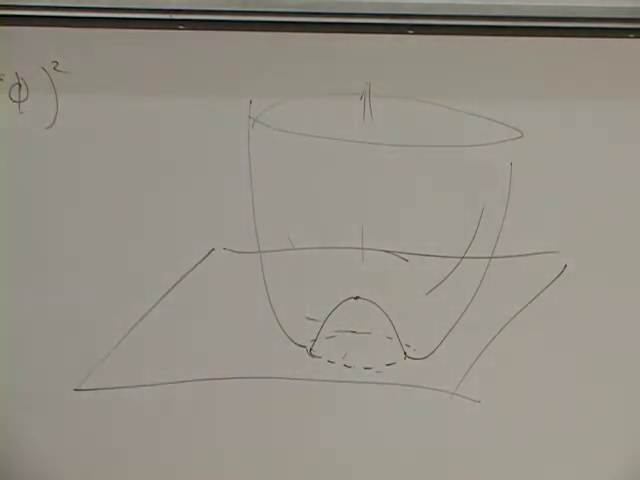
\includegraphics[width=0.72\textwidth]{lecture_07_figure_06.png}
\caption{对称破缺势画成旋转曲面。原点是极不稳定的，简并的极小值构成圆形的谷底。}
\lectureframe{00:37:25}
\end{figure}

把场想象成普通空间每一点处这个内部平面中的一个小箭头。势要求每个箭头的长度为\(f\)。梯度能量要求邻近的箭头指向几乎相同的方向。因此基态在各处都具有相同的角度，但没有任何角度被定律所偏好。这就是连续自发对称破缺。

\section{从畴壁到光滑扭曲}

重复边界实验。在左边界把场固定在一个真空点\(A\)；在右边界把它固定在另一个真空点\(B\)。局域化的跳变会使梯度变得很大。然而，与离散情形不同，场可以在沿圆连续变化的同时始终停留在势的底部。

在低能下把场写成\(\phi=f e^{i\alpha(x)}\)。在一维空间中，相关的能量为
\begin{equation}
  E[\alpha]
  =f^2\int_0^L dx\,\left(\frac{d\alpha}{dx}\right)^2.
  \label{eq:l07-angle-functional}
\end{equation}
对于固定的端点角度，变分给出
\begin{equation}
  \frac{d^2\alpha}{dx^2}=0,
  \qquad
  \alpha(x)=\alpha_A+
    \frac{\alpha_B-\alpha_A}{L}\,x.
  \label{eq:l07-linear-twist}
\end{equation}
最优的构型把扭曲均匀地分布在整个样品中。其能量按
\begin{equation}
  E_{\rm twist}
  =f^2\frac{(\alpha_B-\alpha_A)^2}{L},
  \label{eq:l07-twist-energy}
\end{equation}
标度，因此可以通过增大\(L\)使其变得任意低廉。

\begin{figure}[htbp]
\centering
\begin{adjustbox}{max width=\linewidth}
\begin{tikzpicture}[x=0.95cm,y=0.95cm]
  \begin{scope}
    \draw[->] (0,0) -- (6.2,0) node[right] {$x$};
    \draw[->] (0,0) -- (0,3.5) node[above] {$\alpha(x)$};
    \draw[very thick,blue!70!black] (0.45,0.65) -- (5.7,2.85);
    \fill (0.45,0.65) circle (1.8pt) node[left] {$\alpha_A$};
    \fill (5.7,2.85) circle (1.8pt) node[right] {$\alpha_B$};
    \node at (3.1,-0.65) {physical space};
  \end{scope}
  \begin{scope}[xshift=9.2cm,yshift=1.65cm]
    \draw[thick] (0,0) circle (1.8);
    \fill (1.55,-0.92) circle (1.8pt) node[below right] {$A$};
    \fill (-0.45,1.74) circle (1.8pt) node[above] {$B$};
    \draw[very thick,blue!70!black,-{Latex[length=2.5mm]}]
      (1.55,-0.92) arc[start angle=-31,end angle=104,radius=1.8];
    \node at (0,-2.35) {vacuum circle};
  \end{scope}
\end{tikzpicture}
\end{adjustbox}
\caption{同一低能构型的两种描述。角度在物理空间中线性变化，而场在内部空间中沿着真空圆的短弧变化。}
\end{figure}

\begin{classroomqa}
\audiencequestion{绕圆可以有两种走法。场走哪条路径，它能否被困在较长的那条上？
\lecturetimestamp{00:41:54}}
\lecturerresponse{对于一般的端点，较短的角路径具有较小的梯度，因而能量较低。直径相对的端点使两条最简单的路径简并。通过缓慢移动一个端点制备的构型可能保留额外的绕数并被困在能垒之后，但对于指定的一对普通端点，未扭曲的最短路径就是基态。}
\end{classroomqa}

\begin{classroomqa}
\audiencequestion{路径能否离开谷底、横穿内部，从而整体上变得更短？\lecturetimestamp{00:43:32}}
\lecturerresponse{在低能、长样品的区域中，爬升径向势并不划算。把半径保持在其真空值并让角度线性变化会使有效能量最小，正如上面的变分法计算所示。对于具有特定势的有限系统，可以同时极小化径向和角向运动，但戈德斯通结论涉及的是任意长波极限，在该极限下沿谷底的光滑运动胜出。}
\end{classroomqa}

\begin{classroomqa}
\audiencequestion{如果圆形谷底被倾斜，使得某一个角度更低，会有什么变化？\lecturetimestamp{00:44:33}}
\lecturerresponse{那么对称性被明显破缺。一个点成为真正的基态，沿圆的运动获得回复力，角向激发不再严格无质量。}
\end{classroomqa}

\section{质量作为零动量振荡的代价}

光滑扭曲揭示了一个能量仅来自梯度的场。要理解为什么这意味着无质量粒子，比较相对论色散关系
\begin{equation}
  \omega^2=\bm{k}^2+m^2.
  \label{eq:l07-dispersion}
\end{equation}
波\(e^{i(\bm{k}\cdot\bm{x}-\omega t)}\)携带动量\(\bm{k}\)。如果\(m=0\)，其能量在波长趋于无穷时趋于零：\(\omega=|\bm{k}|\to0\)。如果\(m\ne0\)，空间均匀的模式\(\bm{k}=0\)仍以频率\(\omega=m\)振荡。质量是不可约的零动量能量。

同样的区分在拉格朗日量中可见。一项
\begin{equation}
  -\frac12m^2\varphi^2
\end{equation}
即使对于均匀位移也提供回复力。只有导数项的场没有这样的回复力：使其波长更长，其梯度能量就趋于零。

\subsection{极坐标变量分离出两种模式}

将破缺的复场写为
\begin{equation}
  \phi(x)=\rho(x)e^{i\alpha(x)}.
  \label{eq:l07-polar}
\end{equation}
\(\rho\) 和 \(\alpha\) 都是场。求导给出
\begin{align}
  \partial_\mu\phi
  &=e^{i\alpha}
    \left(\partial_\mu\rho+i\rho\,\partial_\mu\alpha\right),\\
  \partial_\mu\phi^*
  &=e^{-i\alpha}
    \left(\partial_\mu\rho-i\rho\,\partial_\mu\alpha\right).
\end{align}
交叉项相消，剩下
\begin{equation}
  \partial_\mu\phi^*\,\partial^\mu\phi
  =(\partial_\mu\rho)(\partial^\mu\rho)
   +\rho^2(\partial_\mu\alpha)(\partial^\mu\alpha).
  \label{eq:l07-polar-kinetic}
\end{equation}
由于 \(\phi^*\phi=\rho^2\)，
\begin{equation}
  \mathcal L
  =(\partial\rho)^2+\rho^2(\partial\alpha)^2-V(\rho^2).
  \label{eq:l07-polar-lagrangian}
\end{equation}
势中包含 \(\rho\) 但不包含 \(\alpha\)。这种缺失正是该对称性最有用的形式。

\begin{figure}[htbp]
\centering
\includegraphics[width=0.88\textwidth]{lecture_07_figure_03.png}
\caption{极坐标场的拉格朗日量、其加框的低能角向项，以及对称性破缺势。径向运动沿势爬升；角向运动沿谷底行进。}
\lectureframe{00:56:40}
\end{figure}

对于能量极低的激发，场保持在 \(\rho=f\) 附近。于是
\begin{equation}
  \mathcal L_{\rm angular}
  \simeq f^2(\partial_\mu\alpha)(\partial^\mu\alpha).
\end{equation}
将正则归一化的角向场定义为（在 \(1/2\) 因子的约定下）
\begin{equation}
  \beta=\sqrt{2}\,f\alpha,
  \qquad
  \mathcal L_{\rm angular}
  =\frac12(\partial_\mu\beta)(\partial^\mu\beta).
  \label{eq:l07-goldstone-field}
\end{equation}
不存在 \(\beta^2\) 项。该角向场的量子是无质量的。它们就是戈德斯通玻色子。

径向场的行为不同。将 \(\rho\) 同时从 \(f\) 处处移开，它会滚回、越过，并围绕谷底振荡。若 \(\rho=f+h\)，则式 ~\eqref{eq:l07-mexican-hat} 的展开给出
\begin{equation}
  V(f+h)=V(f)+\frac12m_h^2h^2+\cdots,
\end{equation}
因此 \(h\) 是有质量的。从几何上看，角向方向是平坦的，而径向方向是弯曲的。

\begin{classroomqa}
\audiencequestion{如果场被径向移开，它是否只是落回原处，接下来又会发生什么？\lecturetimestamp{00:57:10}}
\lecturerresponse{没有角向运动时，它朝极小值下落、越过，并作径向振荡。均匀振荡具有零空间动量但非零频率；该频率就是径向激发的质量。相比之下，均匀的角向位移落在另一个真空上，且没有回复力。}
\end{classroomqa}

这就是戈德斯通原理在本例中的内容：自发破缺一个连续整体对称性，会为真空流形的每一个独立平坦方向产生一个无质量模式。
\editorialnote{该陈述假定了相对论性场论的通常条件。在非相对论多体系统中，南部--戈德斯通模式的计数和色散可能更为微妙，但本讲的长波长结论对这个相对论性 \(U(1)\) 模型仍然是正确的。}

\section{自旋波、弦与声}

该定理是抽象的，但其机制却为人所熟悉。在各向同性铁磁体中，所有自旋可以一起旋转而不改变能量。让取向在样品中非常缓慢地变化，就得到自旋波。其代价随波数趋于零，因此它是破缺的自旋旋转对称性的戈德斯通模式。

一根长弹性弦提供了另一幅图景。忽略重力，将两端固定，使整根弦可以竖直平移。均匀的竖直平移不耗费能量。让平移沿弦缓慢变化，它就变成一种长波长横波。均匀的对称操作被提升为温和的、依赖于位置的形变。

\begin{figure}[htbp]
\centering
\includegraphics[width=0.68\textwidth]{lecture_07_figure_04.png}
\caption{在戈德斯通模式类比中画出的缓慢变化的弦轮廓。物理要点是长波长形变的小斜率，而不是曲线的竖直位置。}
\lectureframe{01:04:19}
\end{figure}

\begin{classroomqa}
\audiencequestion{弦能否在具有零动量的同时携带振荡能量？\lecturetimestamp{01:04:41}}
\lecturerresponse{必须区分竖直的机械动量与沿弦的波动动量。驻波可以具有零净动量，因为它是 \(+k\) 和 \(-k\) 模式的叠加，同时仍携带能量。在场论类比中，动量指的是沿轴的波数；竖直位移代表内部场坐标。}
\end{classroomqa}

弹簧玩具给出纵向版本。将整个理想化的无限长弹簧玩具沿其轴平移，什么都不会改变。将相邻部分平移略微不同的量，结果就是一种温和的压缩波。在固体或流体中，长波长声波同样源自集体位移和密度变化。自旋波、弦的横波和声并非相同的微观激发，但它们共享决定性的模式：均匀连续操作不耗费能量，而其缓慢变化的版本则成为一种软模式。
\editorialnote{在晶体中，声学声子通常被描述为自发破缺的连续平移的南部--戈德斯通模式。弦和弹簧玩具是本讲中用来揭示同一仅含导数能量结构的力学类比。}

术语的重要性足以开个简短的课堂玩笑：这些是\emph{戈德斯通}玻色子，以杰弗里·戈德斯通命名，而不是规范玻色子。讲义提到戈德斯通是苏斯金德的朋友，然后转向真正不同的主题——规范不变性。

\section{从全局相位对称性到规范对称性}

\(U(1)\)相位对称性在本课程中已经作为与电荷守恒相联系的对称性出现过。带电粒子场是复的，将这样的场乘以一个共同的相位，整体理论保持不变。为直观起见可以使用“电”这个词，尽管该电荷也可能代表另一种\(U(1)\)量子数。真实的光子是无质量的；最终的目标是像光子那样的场，例如有质量的\(Z\)。

新的问题是，当\(\theta\)在时空中任意变化时，
\begin{equation}
  \phi'(x)=e^{i\theta(x)}\phi(x)
  \label{eq:l07-local-u1}
\end{equation}
能否成为一种对称性。函数\(\theta(x)\)是变换参数，而不是额外的动力学场。我们通过求导来检验这一设想：
\begin{equation}
  \partial_\mu\phi'
  =e^{i\theta}
   \left[\partial_\mu\phi+i(\partial_\mu\theta)\phi\right].
  \label{eq:l07-local-derivative}
\end{equation}
当\(\theta\)为常数时，这一额外项不存在。对于共轭场，
\begin{equation}
  \partial_\mu\phi^{*\prime}
  =e^{-i\theta}
   \left[\partial_\mu\phi^*-i(\partial_\mu\theta)\phi^*\right].
\end{equation}
两者之积为
\begin{align}
  \partial_\mu\phi^{*\prime}\partial^\mu\phi'
  ={}&
  \partial_\mu\phi^*\partial^\mu\phi
  i\left(
      \phi\,\partial_\mu\phi^*
      -\phi^*\partial_\mu\phi
    \right)\partial^\mu\theta
  \nonumber\\
  &+\phi^*\phi\,
    \partial_\mu\theta\,\partial^\mu\theta.
  \label{eq:l07-local-failure}
\end{align}
势能项仍然不变，因为\(\phi^*\phi\)不变，但普通的动能项不再成立。全局对称性并没有自动变成局域对称性。

\begin{classroomqa}
\audiencequestion{在墨西哥帽图像中，这种失败是否意味着圆形谷底周围存在隆起？\lecturetimestamp{01:19:37}}
\lecturerresponse{不。势能可以在角方向上保持完全平坦。额外的代价来自相位在不同时空点不同时的梯度。这不是谷底的波纹；而是普通导数项探测到了空间变化。}
\end{classroomqa}

\subsection{补偿矢量场}

自然界的\(W\)、\(Z\)和胶子相互作用是由局域规范对称性组织起来的，而不仅仅是由刚性变换。要使局域相位操作成为对称性，需用一个四维矢量场\(A_\mu\)来扩充理论。在电磁学中，\(A_0\)是标量势，三个空间分量构成矢量势。它们的导数构成电场和磁场。

选择内部自洽的约定
\begin{equation}
  \phi'=e^{i\theta}\phi,
  \qquad
  A'_\mu=A_\mu-\partial_\mu\theta,
  \qquad
  D_\mu=\partial_\mu+iA_\mu.
  \label{eq:l07-gauge-convention}
\end{equation}
在检验抵消时，板书改变了一个符号；式\eqref{eq:l07-gauge-convention}同时固定了全部三个符号。规范耦合和电荷已被暂时吸收进\(A_\mu\)。
\editorialnote{若显式写出电荷\(q\)和耦合\(g\)，可以写为
\(D_\mu=\partial_\mu+igqA_\mu\)和
\(A'_\mu=A_\mu-(gq)^{-1}\partial_\mu\theta\)。讲义省略了这些常数，以使抵消关系保持可见。}

对于共轭场，
\begin{equation}
  D_\mu\phi^*=\partial_\mu\phi^*-iA_\mu\phi^*.
\end{equation}
现在
\begin{align}
  D'_\mu\phi'
  &=
  \left(\partial_\mu+iA'_\mu\right)e^{i\theta}\phi
  \nonumber\\
  &=
  e^{i\theta}
  \left[
    \partial_\mu\phi+i(\partial_\mu\theta)\phi
    +i(A_\mu-\partial_\mu\theta)\phi
  \right]
  \nonumber\\
  &=e^{i\theta}D_\mu\phi.
  \label{eq:l07-covariant-transform}
\end{align}
\(\theta\)不需要的导数项被\(A_\mu\)的变换抵消。同样，
\begin{equation}
  D'_\mu\phi^{*\prime}=e^{-i\theta}D_\mu\phi^*.
\end{equation}
两者之积不变。形容词\emph{协变}意味着该导数的变换方式与场本身一样简单。

\section{规范场的动力学}

仅仅为了修正导数而引入\(A_\mu\)，会使它没有自身的动力学。规范不变的场强为
\begin{equation}
  F_{\mu\nu}
  =\partial_\mu A_\nu-\partial_\nu A_\mu.
  \label{eq:l07-field-strength}
\end{equation}
它是反对称的，因此\(F_{\mu\mu}=0\)。它的时间--空间分量包含电场，而空间--空间分量包含磁场。用熟悉的三维矢量语言来说，电磁能量密度正比于\(\bm E^2+\bm B^2\)，而洛伦兹拉格朗日量正比于\(\bm E^2-\bm B^2\)，符号取决于度规约定。

\begin{classroomqa}
\audiencequestion{电磁场的能量和拉格朗日量是什么？\lecturetimestamp{01:33:20}}
\lecturerresponse{能量由\(E^2+B^2\)构成；拉格朗日量使用\(E^2-B^2\)。协变地，后者写为\(F_{\mu\nu}F^{\mu\nu}\)的常规倍数。反对称张量是矢量势的四维旋度。}
\end{classroomqa}

场强本身是规范不变的：
\begin{align}
  F'_{\mu\nu}
  &=
  \partial_\mu(A_\nu-\partial_\nu\theta)
  -\partial_\nu(A_\mu-\partial_\mu\theta)
  \nonumber\\
  &=
  F_{\mu\nu}
  -\partial_\mu\partial_\nu\theta
  +\partial_\nu\partial_\mu\theta
  =F_{\mu\nu}.
  \label{eq:l07-field-strength-invariant}
\end{align}
最后一个等号成立，是因为普通的混合偏导数可交换。因此，一个标准的规范不变拉格朗日量为
\begin{equation}
  \boxed{
  \mathcal L
  =(D_\mu\phi)^*D^\mu\phi
  -V(\phi^*\phi)
  -\frac14F_{\mu\nu}F^{\mu\nu}}
  \label{eq:l07-scalar-qed}
\end{equation}
直到度规所选的符号和归一化约定。

\begin{figure}[htbp]
\centering
\includegraphics[width=0.84\textwidth]{lecture_07_figure_05.png}
\caption{板书上的协变导数和组装好的规范不变拉格朗日量。那里省略了数值因子，以使变换结构保持可见。}
\lectureframe{01:38:45}
\end{figure}

这一构造将全局\(U(1)\)对称性提升为局域对称性，但这样做是有代价的---或者从物理上说，是得到了一份礼物---：一个新的矢量场。在阿贝尔例子中，该场就是电磁势。

\begin{classroomqa}
\audiencequestion{我们一开始使用的拉格朗日量用的是普通导数。为什么我们有权把它们换成协变导数，并把结果称为真正的理论？\lecturetimestamp{01:42:55}}
\lecturerresponse{我们正在构造一个不同的、扩大的理论：带电物质加上规范场。局域规范不变性决定了它们的耦合。由此得到的量子理论是一个自洽的数学结构，并且与自然界组织光子和弱规范场的方式一致。仅仅不一致地耦合一个相对论性矢量场，会引入非物理的极化并破坏概率，因此规范原理并不是对旧自由标量理论的美化改写。}
\end{classroomqa}

\begin{classroomqa}
\audiencequestion{所以，加入新场就是这一修改的根本理由吗？\lecturetimestamp{01:44:57}}
\lecturerresponse{是的。没有\(A_\mu\)时，局域转动后场的导数含有一个未被抵消的\(\partial_\mu\theta\)。有了\(A_\mu\)及其变换规律，抵消就能成立。用几何语言说，\(A_\mu\)是丛上的一个联络；那套更深刻的数学是真实且有用的，但上面这些代数已经包含了这里所需的部分。}
\end{classroomqa}

\section{为什么裸规范玻色子质量被禁止}

对于普通的玻色场，质量由二次项表示。人们很想加上
\begin{equation}
  \Delta\mathcal L_{\rm Proca}
  =\frac12m^2A_\mu A^\mu.
  \label{eq:l07-proca}
\end{equation}
但在\(A_\mu\mapsto A_\mu-\partial_\mu\theta\)下，
\begin{equation}
  A'_\mu A^{\mu\prime}
  =
  A_\mu A^\mu
  -2A^\mu\partial_\mu\theta
  +\partial_\mu\theta\,\partial^\mu\theta,
\end{equation}
所以式~\eqref{eq:l07-proca}不是规范不变的。我们不能在保留局域对称性的同时，把质量手动塞进这个规范理论。

\begin{figure}[htbp]
\centering
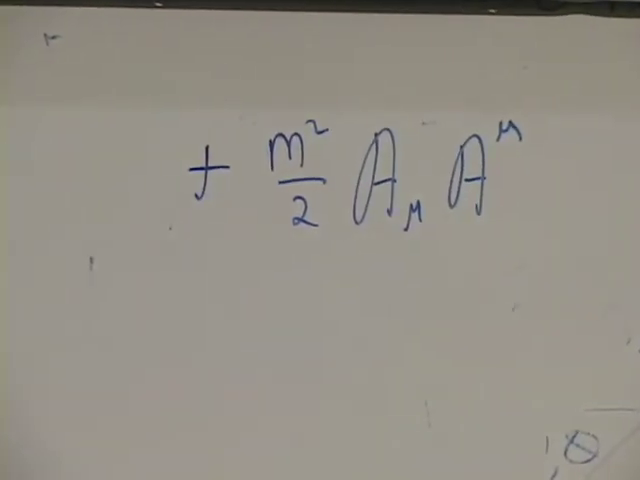
\includegraphics[width=0.72\textwidth]{lecture_07_figure_07.png}
\caption{所提议的裸矢量质量
\(\tfrac12m^2A_\mu A^\mu\)。它在\(A_\mu\mapsto A_\mu-\partial_\mu\theta\)下的失效，正是引出希格斯机制的那个障碍。}
\lectureframe{01:39:48}
\end{figure}

这就是表面上的僵局。规范不变性解释了无质量的光子，并保护理论免于非物理的自由度，但\(W\)和\(Z\)是有质量的。出路不可能是显式的矢量质量。它必须来自一个规范不变拉格朗日量中已经存在的场。

\begin{classroomqa}
\audiencequestion{引入规范不变性本身会产生戈德斯通玻色子吗？\lecturetimestamp{01:45:51}}
\lecturerresponse{不会。戈德斯通玻色子是在引入矢量势之前，一个连续的\emph{整体}对称性被自发破缺时出现的。一旦对称性成为局域的，变化的相位就可以由\(A_\mu\)来补偿。在破缺的规范理论中，角向模式不再是一个独立的无质量粒子；它为如今有质量的矢量场提供了额外的极化。下一讲将推导这一陈述，而不是仅仅宣布它。}
\end{classroomqa}

\begin{classroomqa}
\audiencequestion{这些能解释河流为什么蜿蜒吗？\lecturetimestamp{01:47:03}}
\lecturerresponse{这里不知道有什么直接联系。流体涡旋乃至生物体的形状当然都可以用对称性方法来描述，而且人们永远不该惊讶于在意外之处发现场论思想，但本讲并不主张存在关于河流蜿蜒的规范理论。}
\end{classroomqa}

\section{本讲止于何处}

我们现在已经具备了一开始承诺的两个要素。一个具有真空圆环的连续整体对称性有一条平坦的角向方向，其缓慢变化就是一个无质量的戈德斯通场。局域对称性要求一个规范联络和协变导数，并且禁止式~\eqref{eq:l07-proca}中直接的矢量质量。

下一步是把式~\eqref{eq:l07-mexican-hat}的破缺势用于式~\eqref{eq:l07-scalar-qed}的规范不变理论之中。于是两件事同时发生：单独的戈德斯通粒子从物理谱中消失，而矢量场获得质量。在通常的教学语言中，规范对称性被自发破缺；更准确地说，规范冗余仍然存在，而理论进入一个带有有质量矢量激发的希格斯相。\editorialnote{局域规范对称性是描述上的冗余，而不是作用于不同可观测态之间的普通物理对称性。本讲使用了自发规范对称性破缺这一标准简写。规范不变的物理陈述是希格斯相中自由度的重新组合。}

这就是希格斯现象。我们还没有执行它。本讲完成了必要的更艰难的工作，使问题足够精确，以至于当解答到来时，它将是不可避免的。
